
\documentclass[11pt]{report}

\usepackage{graphicx}
\usepackage{framed}
%\graphicspath{ {images/} }

\marginparwidth 0.5in 
\oddsidemargin 0.25in 
\evensidemargin 0.25in 
\marginparsep 0.25in
\topmargin 0.0in 
\textwidth 6in \textheight 8.5in

\title{sQuire: A Web Based Collaborative Editor}
\author{bolt1003, wern0096, alsh5301, sass8427, dani2918, boss2849, snev7821, jank6275}

\begin{document}
\maketitle

\tableofcontents

\chapter{Application Domain Specification}

\section{Program Premise}
\begin{figure}[h!]
\caption{Squire will be a web-based collaborative integrated development environment with a project development center. Squire will allow multiple users to edit files and communicate in real time. First, projects are stubbed out by a user and then other users can join and/or vote to support for their favorite projects. After a certain amount of support, planning, and documentation is reached for a project, the project becomes a fully fleged project and then community development can start. Think kickstarter for code where people pledge their help with the project and not just money.}
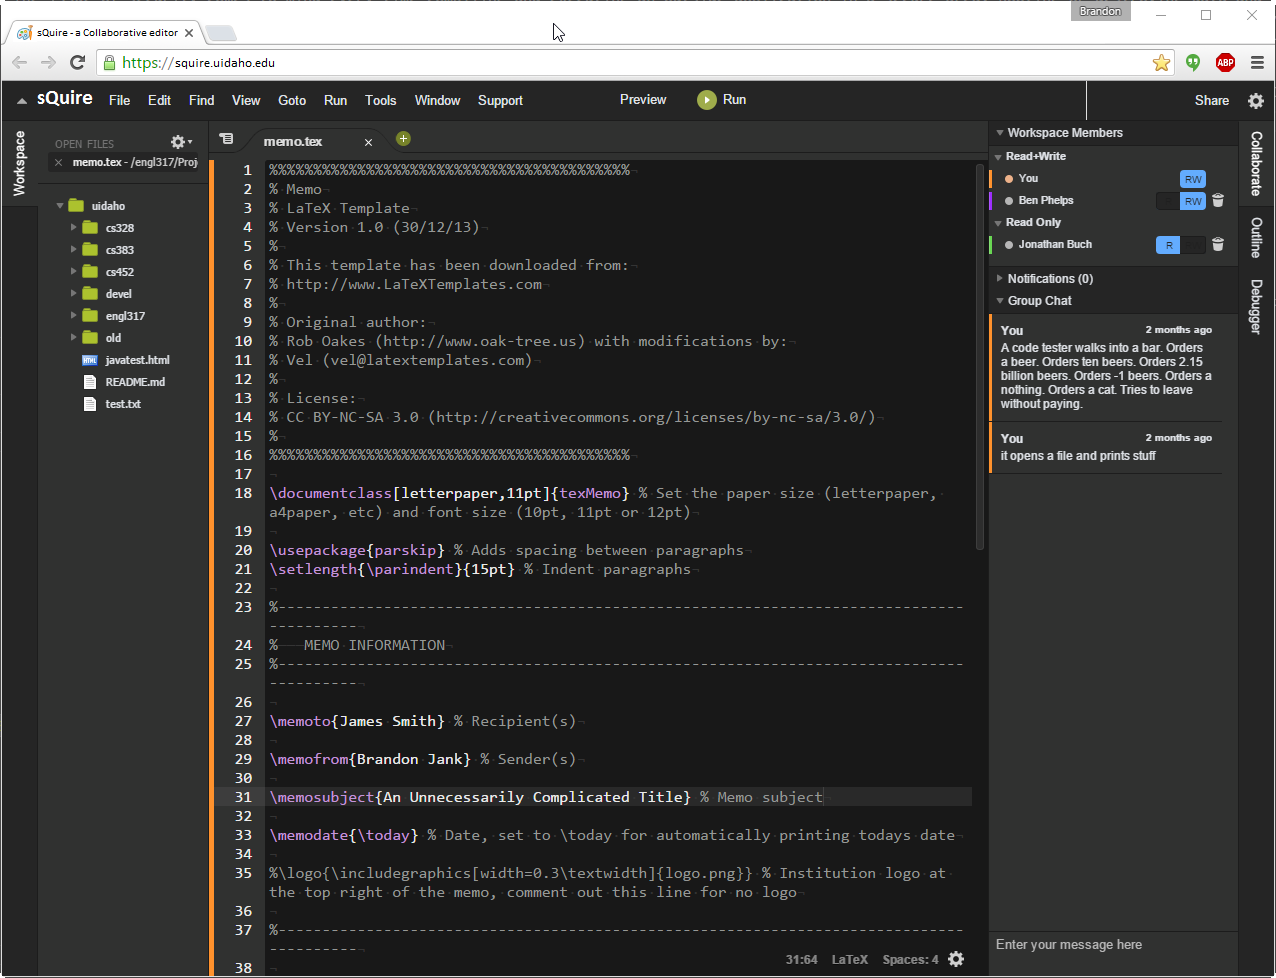
\includegraphics[width=0.7\textwidth]{squire}
\end{figure}



\section{Use Case Diagrams}
\subsection{Overview (jank6275)}
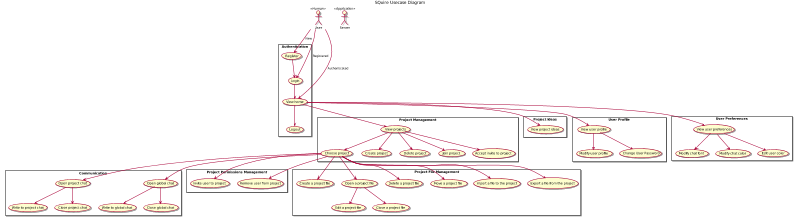
\includegraphics[width=\textwidth]{diagrams/overview-jank6275}
A usecase diagram that shows all of sQuire\'s features.

\subsection{Project Ideas (dani2918)}
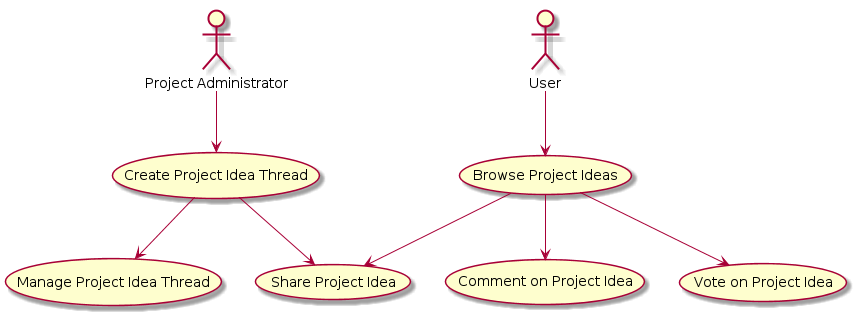
\includegraphics[width=\textwidth]{diagrams/dani2918}

\subsection{Authentication (alsh5301)}
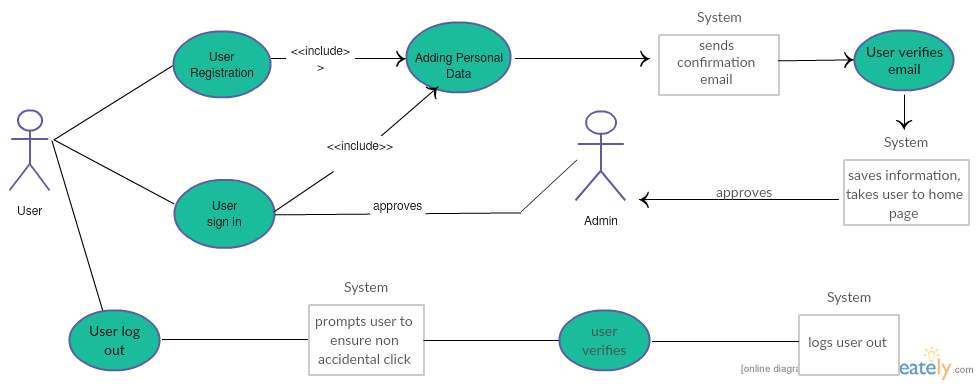
\includegraphics[width=\textwidth]{alsh5301_UserRegistration}

\subsection{Communication (jank6275)}
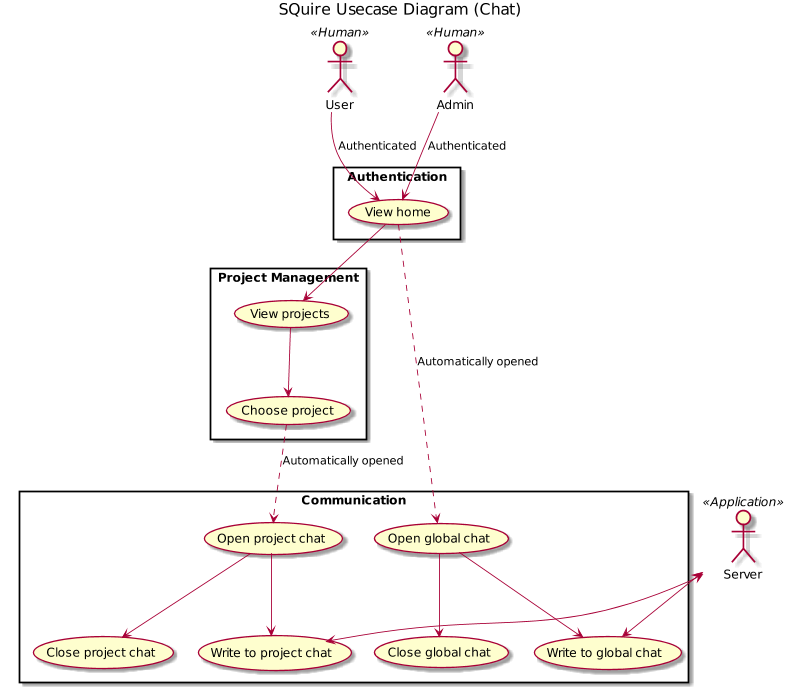
\includegraphics[width=\textwidth]{diagrams/jank6275}
A usecase diagram for sQuire\'s communication features.

\subsection{File Editing (wern0096)}
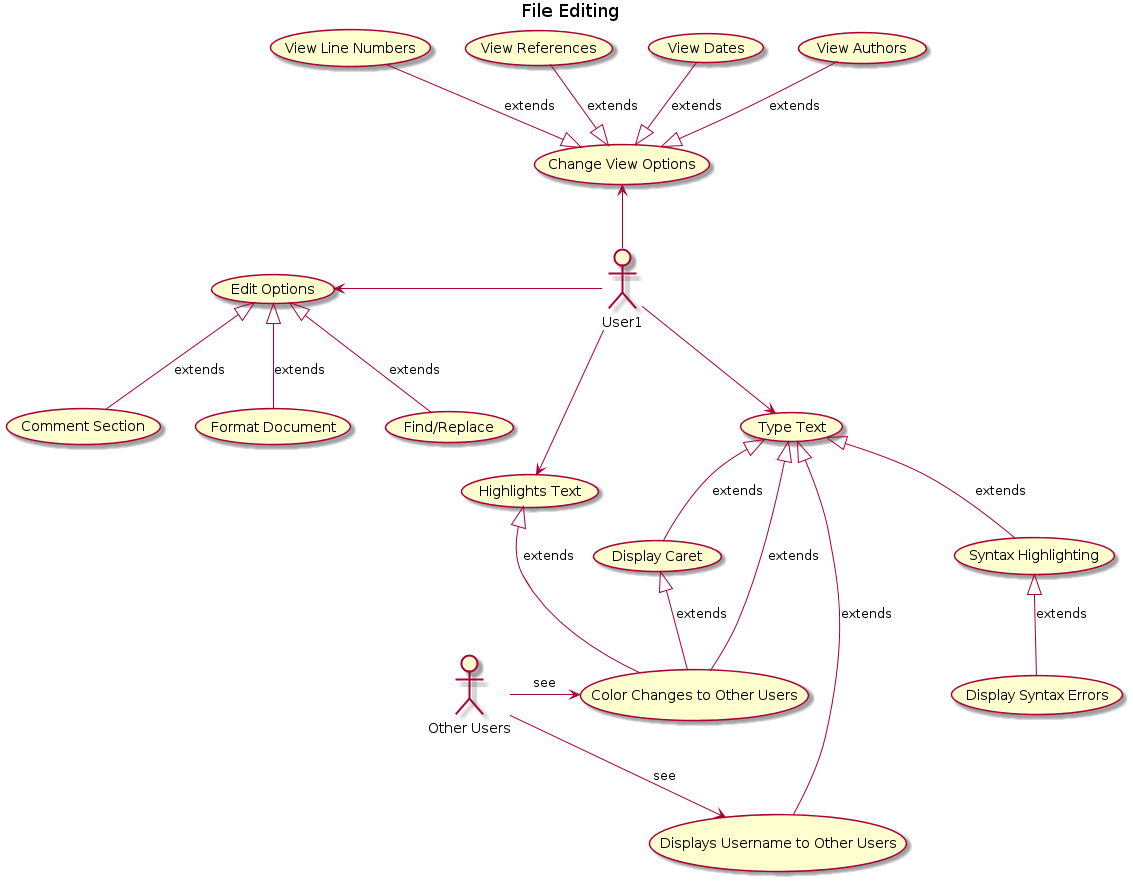
\includegraphics[width=\textwidth]{diagrams/wern0096-FileEditing}

\subsection{File Management (wern0096)}
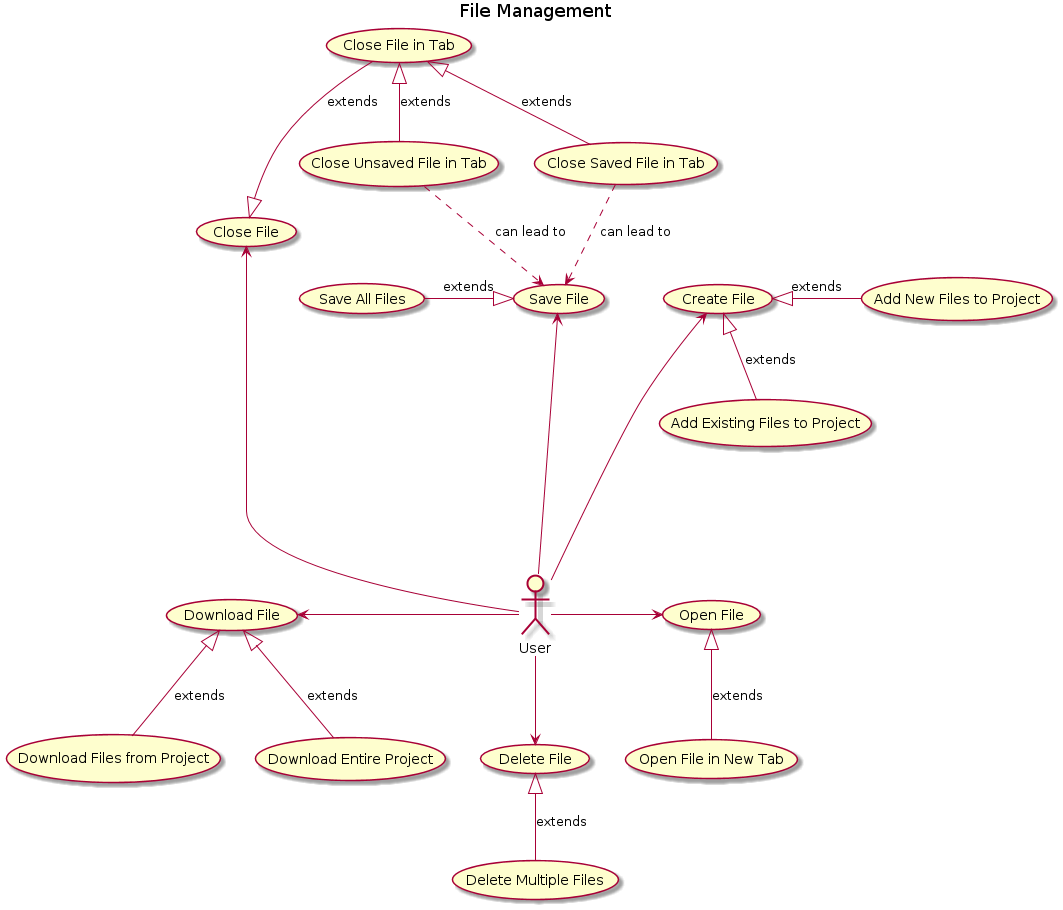
\includegraphics[width=\textwidth]{diagrams/wern0096-FileManagement}

\subsection{Project Management (sass8427)}
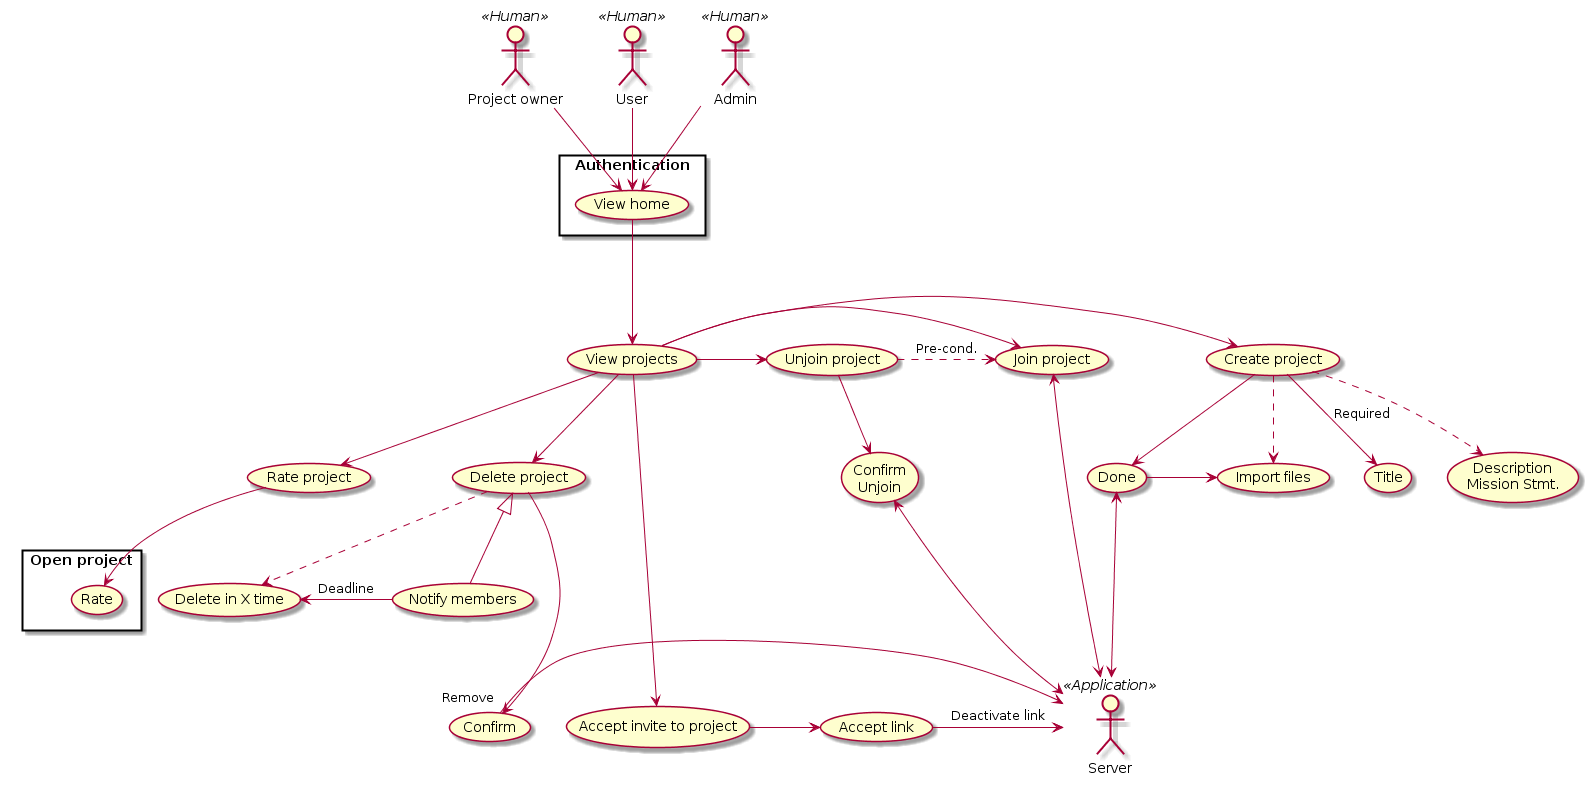
\includegraphics[width=\textwidth]{sass8427}

\subsection{User Profile Management (bolt1003)}
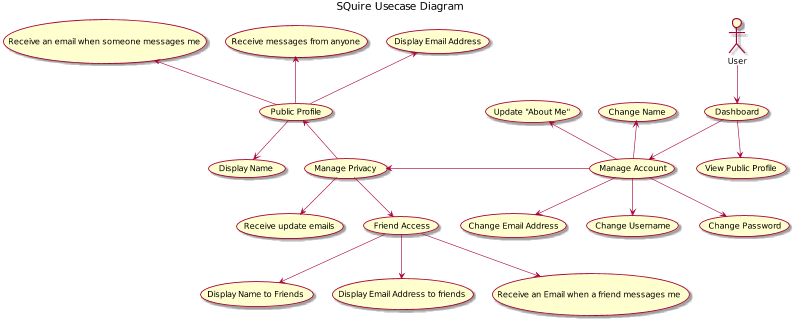
\includegraphics[width=\textwidth]{diagrams/bolt1003}

\subsection{Project User Management (boss2849)} 
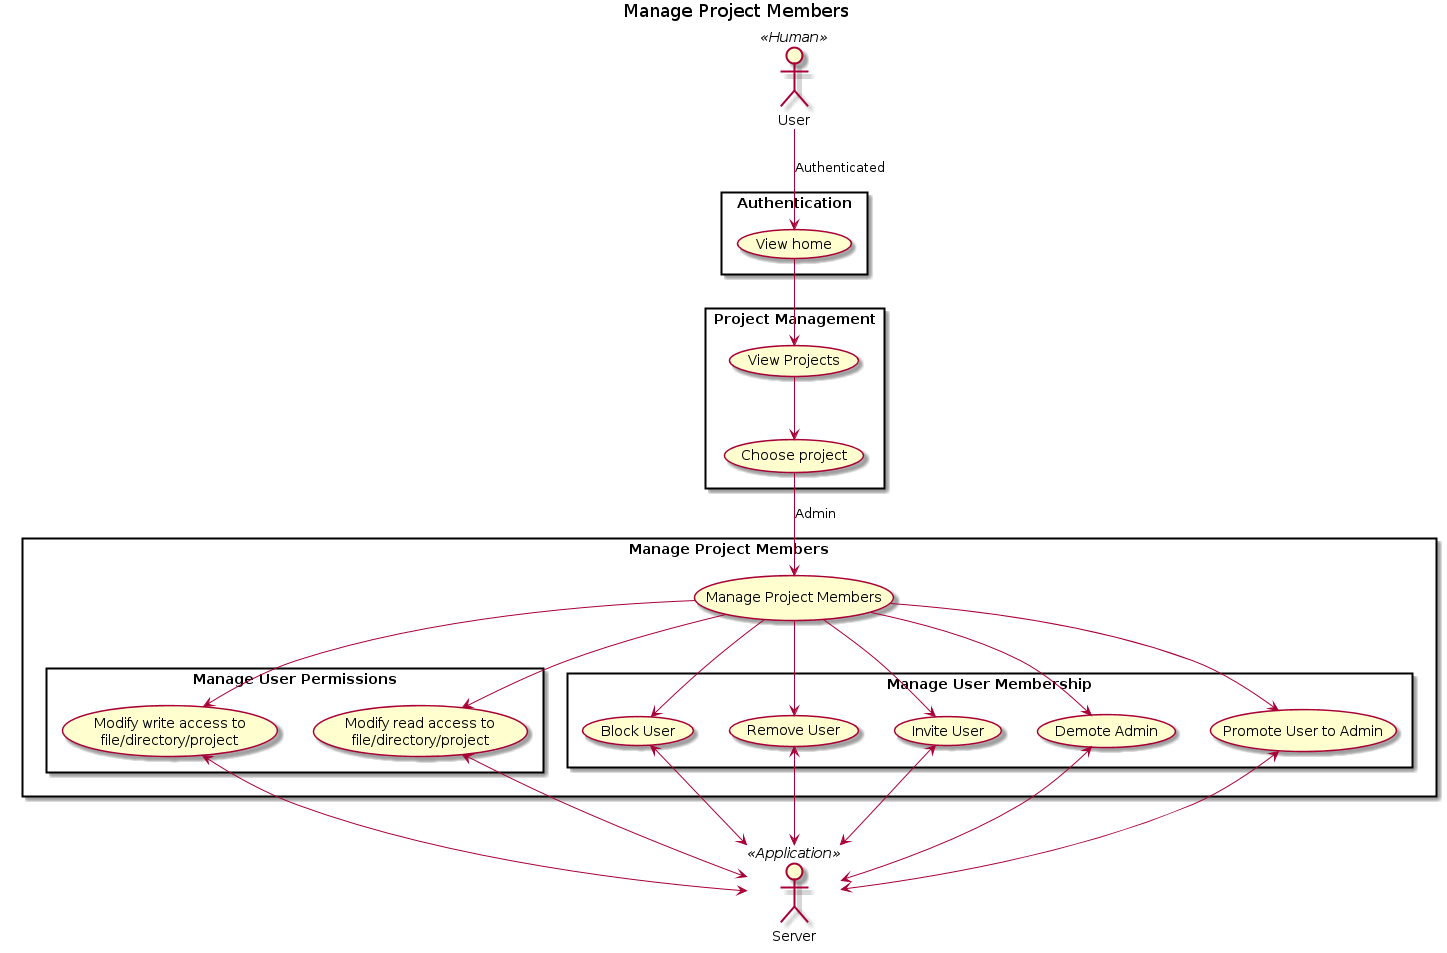
\includegraphics[width=\textwidth]{diagrams/boss2849}

\subsection{User Editor Preferences (snev7821)}
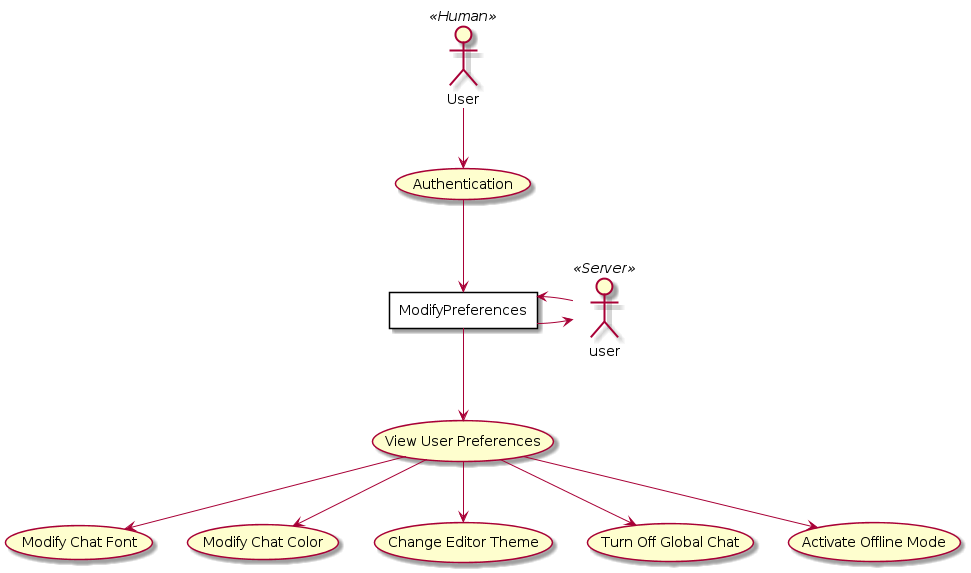
\includegraphics[width=\textwidth]{diagrams/snev7821}



\section{Use Case Descriptions}

\subsection{Authentication (alsh5301)}
\subsubsection{Sign up (alsh5301)}
\begin{tabular}{ p{2cm} p{12cm} }
 \hline
 \\
 \textit{Actors:} & user. \\ 
 \\
 \textit{Goals:} & To register and create an account in the program. \\
 \\
 \textit{Pre-conditions:} & None. \\
 \\
 \textit{Summary:} & The user signs up and creates an account using their email address and creates username and password. Once they can access to the program. \\ 
 \\
 \textit{Related use cases:} & None. \\ 
 \\
 \textit{Steps:} & \begin{enumerate}
  \item User is prompted to enter email and password. 
  \item System sends confirmation email. 
  \item User verifies email. 
  \item User clicks finish System presents user with additional info page. 
  \item User enters password, may choose to upload photo, works, etc. 
  \item System saves information, takes user to home page. 
 \end{enumerate} \\
 \\
 \textit{Alternative 1:} & User already has an account. \\ 
 \\
 \textit{Alternative 2:} & User doesn't confirm email. Delete request after timeout period. \\
 \\
\hline
\end{tabular}

\subsubsection{Sign in (alsh5301)}
\begin{tabular}{ p{2cm} p{12cm} }
 \hline
 \\
 \textit{Actors:} & Users. \\ 
 \\
 \textit{Goals:} & Pre-existing user signs into profile. \\
 \\
\textit{Precondition:} & User must already have an account \\
\\
\textit{Summary:} & User wishes to access their account, projects and info. \\
\\
 \textit{Steps:} & \begin{enumerate}
  \item User is prompted to enter email and password 
  \item System verifies information
  \item If info is correct user is presented with their home page. 
  \item If user forgot their user name, they can click "Forgot Username button. They then input their email address.
  \item System validates their email address with an account, and sends an email with the username  
  \item If user forgot their password, they click "Forgot password" button. Then they input their email address.
  \item System validates their email address with an account, and sends an email to them with a temporary password.
 \end{enumerate} \\
 \\
 \textit{Alternatives:} & Information is incorrect, user tries again. Or makes a new account \\
 \\
\hline
\end{tabular}

\subsubsection{Logout (alsh5301)}
\begin{tabular}{ p{2cm} p{12cm} }
 \hline
 \\
 \textit{Actors:} & Users. \\ 
  \\
 \textit{Goal:} & Existing user logs out \\ 
 \\
 \textit{Precondition:} & User must be logged in \\
 \\
 \textit{Summary:}  & The user can log-out of the program after finishing process the project  \\
 \\
 \textit{Steps:} & \begin{enumerate}
 \item User clicks the "log-out" button. 
 \item System prompts user to ensure non-accidental click. 
 \item User verifies. 
 \item System logs user out. 
 \item User enters password, may choose to upload photo, works, etc. 
 \item System saves information, takes user to home page.
 \end{enumerate} \\
\\
  \textit{Alternative 1:} & The program will send notification to ask if the user is sure to sign out. \\
  \textit{Alternative 2:} & user cancels on step two. Return to home page. \\ 
 \\
\hline
\end{tabular}



\subsection{Project Ideas (dani2918)}
\subsubsection{Browse Project Ideas (dani2918)}
\begin{tabular}{ p{2cm} p{12cm} }
 \hline
 \\
 \textit{Actors:} & User \\ 
 \\
 \textit{Goals:} & Examine a list of available project ideas  \\
 \\
 \textit{Pre-conditions:} & User is signed in  \\
 \\
 \textit{Summary:} & User looks through posted project ideas to find projects to work on/discuss \\ 
 \\
 \textit{Related use cases:} & Comment on Project Idea, Vote on Project Idea, Share Project Idea \\ 
 \\
 \textit{Steps:} & \begin{enumerate}
  \item Actor selects Browse Project Ideas button
  \item Actor refines search by selecting from list of project categories as desired
  \item Actor enters terms into search field as desired and views a list of top projects
  \item Actor selects desired project
  \item System displays detailed project information
 \end{enumerate} \\
 \\
 \textit{Alternatives:} & None. \\
 \\
 \textit{Post-conditions:} & None. \\
 \\
\hline
\end{tabular}

\subsubsection{Create Project Idea Thread (dani2918)}
\begin{tabular}{ p{2cm} p{12cm} }
 \hline
 \\
 \textit{Actors:} & Project Administrator \\ 
 \\
 \textit{Goals:} & Generate public interest in project idea  \\
 \\
 \textit{Pre-conditions:} & Prospective project administrator is signed in  \\
 \\
 \textit{Summary:} &  A user with interest in heading up own project can post ideas to get feedback and/or recruit collaborators \\ 
 \\
 \textit{Related use cases:} & Manage Project Idea Thread \\ 
 \\
 \textit{Steps:} & \begin{enumerate}
  \item Actor selects Create Project Idea button
  \item Actor enters prospective project title and thoughts and ideas as a description
  \item Actor selects Submit button

 \end{enumerate} \\
 \\
 \textit{Alternatives:} & None. \\
 \\
 \textit{Post-conditions:} & None. \\
 \\
\hline
\end{tabular}

\subsubsection{Manage Project Idea Thread (dani2918)}
\begin{tabular}{ p{2cm} p{12cm} }
 \hline
 \\
 \textit{Actors:} & Project Administrator \\ 
 \\
 \textit{Goals:} & Respond to feedback and manage project idea  \\
 \\
 \textit{Pre-conditions:} & Prospective project administrator is signed in and has navigated to one of his or her own project threads  \\
 \\
 \textit{Summary:} &  A prospective project administrator responds to others' questions/comments \\ 
 \\
 \textit{Related use cases:} & Create Project Idea Thread \\ 
 \\
 \textit{Steps:} & \begin{enumerate}
  \item Actor selects Reply button on a comment
  \item Actor types feedback to other user
  \item Actor selects Submit button 
  \item System shows confirmation that feedback was received 
  
 \end{enumerate} \\
 \\
 \textit{Alternatives:} & Actor selects Delete Comment instead of Reply to remove harmful feedback. \\
 \\
 \textit{Post-conditions:} & None. \\
 \\
\hline
\end{tabular}

\subsubsection{Comment on Project Idea (dani2918)}
\begin{tabular}{ p{2cm} p{12cm} }
 \hline
 \\
 \textit{Actors:} & User \\ 
 \\
 \textit{Goals:} & Provide detailed feedback on project ideas  \\
 \\
 \textit{Pre-conditions:} & Actor is signed in, has navigated to a project idea  \\
 \\
 \textit{Summary:} &  User provides feedback to or asks questions about a prospective project. \\ 
 \\
 \textit{Related use cases:} & Browse Project Ideas, Vote on Project Idea, Manage Project Idea Thread \\ 
 \\
 \textit{Steps:} & \begin{enumerate}
  \item Actor selects Comment button
  \item Actor types feedback into field 
  \item Actor clicks Submit button
  \item System shows confirmation that feedback was received 
 \end{enumerate} \\
 \\
 \textit{Alternatives:} & None \\
 \\
 \textit{Post-conditions:} & None. \\
 \\
\hline 
\end{tabular}

\subsubsection{Vote on Project Idea (dani2918)}
\begin{tabular}{ p{2cm} p{12cm} }
 \hline
 \\
 \textit{Actors:} & User \\ 
 \\
 \textit{Goals:} & Support promising project ideas or offer criticism to unfavorable ones  \\
 \\
 \textit{Pre-conditions:} & Actor is signed in, has navigated to a project idea  \\
 \\
 \textit{Summary:} &  User offers support/discourages a project idea so that prospective project administrators get feedback and promising project ideas get publicity \\ 
 \\
 \textit{Related use cases:} & Comment on Project Idea \\ 
 \\
 \textit{Steps:} & \begin{enumerate}
  \item Actor selects and Up Vote or Down Vote button
  \item Actor selects Submit button 
  \item System highlights which button the user has selected
 \end{enumerate} \\
 \\
 \textit{Alternatives:} & None \\
 \\
 \textit{Post-conditions:} & None. \\
 \\
\hline
\end{tabular}

\subsubsection{Share Project Idea (dani2918)}
\begin{tabular}{ p{2cm} p{12cm} }
 \hline
 \\
 \textit{Actors:} & User, Project Administrator \\ 
 \\
 \textit{Goals:} & Generate excitement about a project  \\
 \\
 \textit{Pre-conditions:} & Actor is signed in, has navigated to a project idea  \\
 \\
 \textit{Summary:} &  Prospective project administrators or users show other users which projects they believe are worthwhile \\ 
 \\
 \textit{Related use cases:} & Comment on Project Idea \\ 
 \\
 \textit{Steps:} & \begin{enumerate}
  \item Actor selects Share button
  \item Actor selects an audience and method with which to share selected project
  \item Actor selects Submit button
  \item System notifies or shows audience the shared project idea
 \end{enumerate} \\
 \\
 \textit{Alternatives:} & None \\
 \\
 \textit{Post-conditions:} & None. \\
 \\
\hline
\end{tabular}



\subsection{Communication (jank6275)}
\subsubsection{Open project chat (jank6275)}
\begin{tabular}{ p{2cm} p{12cm} }
 \hline
 \\
 \textit{Actors:} & User \\ 
 \\
 \textit{Goals:} & To open the project chat window. \\
 \\
 \textit{Pre-conditions:} & User must be registered, signed in, and have a open project.  \\
 \\
 \textit{Summary:} & User opens a project and the project chat automatically opens. The chat window displays chat history and updates when new chat messages are received. \\ 
 \\
 \textit{Related use cases:} & Join global chat. \\ 
 \\
 \textit{Steps:} & \begin{enumerate}
  \item User opens a project.
  \item Chat is notified that user has joined.
  \item System displays project chat window to the user.
 \end{enumerate} \\
 \\
 \textit{Alternatives:} & None. \\
 \\
 \textit{Post-conditions:} & None. \\
 \\
\hline
\end{tabular}

\subsubsection{Open global chat (jank6275)}
\begin{tabular}{ p{2cm} p{12cm} }
 \hline
 \\
 \textit{Actors:} & User \\ 
 \\
 \textit{Goals:} & To open the global chat window. \\
 \\
 \textit{Pre-conditions:} & User must be registered, signed in, and anywhere on website.  \\
 \\
 \textit{Summary:} & User authenticates with the server and the global chat automatically opens. The chat window displays chat history and updates when new chat messages are received.  \\ 
 \\
 \textit{Related use cases:} & Join project chat. \\ 
 \\
 \textit{Steps:} & \begin{enumerate}
  \item User clicks open global chat.
  \item Chat is notified that user has joined.
  \item System displays global chat window.
 \end{enumerate} \\
 \\
 \textit{Alternatives:} & None. \\
 \\
 \textit{Post-conditions:} & None. \\
 \\
\hline
\end{tabular}

\subsubsection{Close project chat (jank6275)}
\begin{tabular}{ p{2cm} p{12cm} }
 \hline
 \\
 \textit{Actors:} & User \\ 
 \\
 \textit{Goals:} & To close the project chat window. \\
 \\
 \textit{Pre-conditions:} & User must be registered, signed in, and in editor Mode.  \\
 \\
 \textit{Summary:} & User clicks on close project chat and the chat window closes. \\ 
 \\
 \textit{Related use cases:} & Close global chat. \\ 
 \\
 \textit{Steps:} & \begin{enumerate}
  \item User clicks close project chat.
  \item Chat is notified that user has left.
  \item Client closes project chat window.
 \end{enumerate} \\
 \\
 \textit{Alternatives:} & None. \\
 \\
 \textit{Post-conditions:} & None. \\
 \\
\hline
\end{tabular}

\subsubsection{Close global chat (jank6275)}
\begin{tabular}{ p{2cm} p{12cm} }
 \hline
 \\
 \textit{Actors:} & User \\ 
 \\
 \textit{Goals:} & To close the global chat window. \\
 \\
 \textit{Pre-conditions:} & User must be registered, signed in, and anywhere on website.  \\
 \\
 \textit{Summary:} & User clicks on open global chat and the chat opens, displaying chat history and updating when needed. \\ 
 \\
 \textit{Related use cases:} & Close project chat. \\ 
 \\
 \textit{Steps:} & \begin{enumerate}
  \item User clicks close global chat.
  \item Chat is notified that user has left.
  \item Client closes global chat window.
 \end{enumerate} \\
 \\
 \textit{Alternatives:} & None. \\
 \\
 \textit{Post-conditions:} & None. \\
 \\
\hline
\end{tabular}

\subsubsection{Write to project chat (jank6275)}
\begin{tabular}{ p{2cm} p{12cm} }
 \hline
 \\
 \textit{Actors:} & User \\ 
 \\
 \textit{Goals:} & To send text to project chat. \\
 \\
 \textit{Pre-conditions:} & User must be registered, signed in, a project opened, with the project chat window open, and the text box selected.  \\
 \\
 \textit{Summary:} & User clicks in the project chat text box and then types a message then either presses enter or clicks the submit button. The text is displayed to all users in the chat, including the user. \\ 
 \\
 \textit{Related use cases:} & Write to global chat. \\ 
 \\
 \textit{Steps:} & \begin{enumerate}
  \item User clicks in the project chat box.
  \item User types a message and then presses enter or clicks submit button.
  \item Message is relayed to all clients with project chat open.
  \item Message is displayed.
 \end{enumerate} \\
 \\
 \textit{Alternatives:} & None. \\
 \\
 \textit{Post-conditions:} & None. \\
 \\
\hline
\end{tabular}

\subsubsection{Write to global chat (jank6275)}
\begin{tabular}{ p{2cm} p{12cm} }
 \hline
 \\
 \textit{Actors:} & User \\ 
 \\
 \textit{Goals:} & To send text to global chat. \\
 \\
 \textit{Pre-conditions:} & User must be registered, signed in, anywhere on website, with the global chat window open, and the text box selected.  \\
 \\
 \textit{Summary:} & User clicks in the global chat text box and then types a message then either presses enter or clicks the submit button. The text is displayed to all users in the chat, including the user. \\ 
 \\
 \textit{Related use cases:} & Write to project chat. \\ 
 \\
 \textit{Steps:} & \begin{enumerate}
  \item User clicks in the global chat box.
  \item User types a message and then presses enter or clicks submit button.
  \item Message is relayed to all clients with global chat open.
  \item Message is displayed.
 \end{enumerate} \\
 \\
 \textit{Alternatives:} & None. \\
 \\
 \textit{Post-conditions:} & None. \\
 \\
\hline
\end{tabular}

\subsubsection{Modify chat font (jank6275)}
\begin{tabular}{ p{2cm} p{12cm} }
 \hline
 \\
 \textit{Actors:} & User \\ 
 \\
 \textit{Goals:} & To change a users font style inside the global and project chat. \\
 \\
 \textit{Pre-conditions:} & User must be registered, signed in, the user settings window opened, and the chat settings tab open.  \\
 \\
 \textit{Summary:} & The user clicks the settings menu and changes their font style for both the project and global chat through a drop down box of available fonts. \\ 
 \\
 \textit{Related use cases:} & Modify chat color. \\ 
 \\
 \textit{Steps:} & \begin{enumerate}
  \item User clicks the settings menu.
  \item User clicks chat settings tab.
  \item User clicks chat font drop down box.
  \item User clicks desired font.
  \item User clicks save.
  \item The user\'s selection is saved in the database.
  \item All further chat messages will use the selected font.
 \end{enumerate} \\
 \\
 \textit{Alternatives:} & None. \\
 \\
 \textit{Post-conditions:} & None. \\
 \\
\hline
\end{tabular}

\subsubsection{Modify chat color (jank6275)}
\begin{tabular}{ p{2cm} p{12cm} }
 \hline
 \\
 \textit{Actors:} & User \\ 
 \\
 \textit{Goals:} & To change a users font color inside the global and project chat. \\
 \\
 \textit{Pre-conditions:} & User must be registered, signed in, the user settings window opened, and the chat settings tab open.  \\
 \\
 \textit{Summary:} & The user clicks the settings menu and changes their font color for both the project and global chat through a drop down box of available colors. \\ 
 \\
 \textit{Related use cases:} & Modify chat font. \\ 
 \\
 \textit{Steps:} & \begin{enumerate}
  \item User clicks the settings menu.
  \item User clicks chat settings tab.
  \item User clicks chat color drop down box.
  \item User clicks desired color.
  \item User clicks save.
  \item The user\'s selection is saved in the database.
  \item All further chat messages from the user will use the selected color.
 \end{enumerate} \\
 \\
 \textit{Alternatives:} & None. \\
 \\
 \textit{Post-conditions:} & None. \\
 \\
\hline
\end{tabular}



\newpage

\subsection{File Management (wern0096)}
\subsubsection{Add New File to Project (wern0096)}
\begin{framed}
	\noindent\textbf{Task Name:} Add New File to Project \\ \\
	\textbf{Task Category:} File Management \\ \\
	\textbf{Actor:} User \\ \\
	\textbf{Summary:} The user performs this task to add a new file to the project. \\ \\
	\textbf{Preconditions:} 
	\begin{enumerate}
		\item User must be registered.
		\item User must be logged in.
		\item User must have a project open.
	\end{enumerate}
	\textbf{Steps:}
	\begin{enumerate}
		\item User clicks \textit{File} in the top menu bar.
		\item System opens a drop-down menu.
		\item User navigates to \textit{Add} -$>$ \textit{New File}.
		\item System opens an \textit{Add New File} dialog window.
		\item User selects the file type and names the file.
		\item User clicks \textit{Add}.
		\item System adds the file to the project.
	\end{enumerate}
	\textbf{Alternatives:} 
	\begin{enumerate}
		\item Step 1: The user right clicks in the project pane and the system continues on to step 2 above.
		\item Step 5: The user clicks \textit{Cancel} and a new file is not added to the project.
	\end{enumerate}
	\textbf{Postconditions:}
	\begin{enumerate}
		\item A new file is added to the project.
		\item The database is updated to reflect the changes.
	\end{enumerate}
	\textbf{Related:} Add Existing File to Project
\end{framed} 

\newpage

\subsubsection{Add Existing File to Project (wern0096)}
\begin{framed}
	\noindent\textbf{Task Name:} Add Existing File to Project \\ \\
	\textbf{Task Category:} File Management \\ \\
	\textbf{Actor:} User \\ \\
	\textbf{Summary:} The user performs this task to add an existing file to the project. \\ \\
	\textbf{Preconditions:} 
	\begin{enumerate}
		\item User must be registered.
		\item User must be logged in.
		\item User must have a project open.
	\end{enumerate}
	\textbf{Steps:}
	\begin{enumerate}
		\item User clicks \textit{File} in the top menu bar.
		\item System opens a drop-down menu.
		\item User navigates to \textit{Add} -$>$ \textit{Existing File}.
		\item System opens an \textit{Add Existing File} dialog window.
		\item User selects \textit{PC} or \textit{SQuire} or \textit{Github}.
		\item System updates the dialog to reflect the selected source.
		\item User navigates to the file's location and selects it.
		\item User clicks \textit{Add}.
		\item System adds the file to the project.
	\end{enumerate}
	\textbf{Alternatives:} 
	\begin{enumerate}
		\item Step 1: The user right clicks in the project pane and the system continues on to step 2 above.
		\item Step 5-7: The user clicks \textit{Cancel} and a new file is not added to the project.
	\end{enumerate}
	\textbf{Postconditions:}
	\begin{enumerate}
		\item An existing file is added to the project.
		\item The database is updated to reflect the changes.
	\end{enumerate}
	\textbf{Related:} Add New File to Project
\end{framed} 

\newpage

\subsubsection{Delete File (wern0096)}
\begin{framed}
	\noindent\textbf{Task Name:} Delete File \\ \\
	\textbf{Task Category:} File Management \\ \\
	\textbf{Actor:} User \\ \\
	\textbf{Summary:} The user performs this task to delete a file from the project. \\ \\
	\textbf{Preconditions:} 
	\begin{enumerate}
		\item User must be registered.
		\item User must be logged in.
		\item User must have a project open.
		\item Current project must have at least one file.
	\end{enumerate}
	\textbf{Steps:}
	\begin{enumerate}
		\item User clicks right clicks a file in the project pane.
		\item System opens a drop-down menu.
		\item User navigates to \textit{Delete}.
		\item System opens an \textit{Delete File} dialog window, asking if the user is sure.
		\item User selects \textit{Yes}.
		\item System deletes the file from the project.
	\end{enumerate}
	\textbf{Alternatives:} 
	\begin{enumerate}
		\item Step 5: The user clicks \textit{Cancel} instead and the file is not deleted from the project.
		\item The user selects multiple files before step 1.
	\end{enumerate}
	\textbf{Postconditions:}
	\begin{enumerate}
		\item The file is deleted from the project.
		\item The database is updated to reflect the changes.
	\end{enumerate}
\end{framed} 

\newpage

\subsubsection{Export Project (wern0096)}
\begin{framed}
	\noindent\textbf{Task Name:} Export Project \\ \\
	\textbf{Task Category:} File Management \\ \\
	\textbf{Actor:} User \\ \\
	\textbf{Summary:} The user performs this task to download a project as a zip file. \\ \\
	\textbf{Preconditions:} 
	\begin{enumerate}
		\item User must be registered.
		\item User must be logged in.
		\item User must have a project open.
		\item User must have download permissions.
	\end{enumerate}
	\textbf{Steps:}
	\begin{enumerate}
		\item User clicks \textit{File} in the top menu bar.
		\item System opens a drop-down menu.
		\item User navigates to \textit{Export} -$>$ \textit{Project}.
		\item System opens an \textit{Export} dialog window.
		\item User navigates to the export location.
		\item User clicks \textit{Export}.
		\item System zips the file and downloads it to the specified location.
	\end{enumerate}
	\textbf{Alternatives:} 
	\begin{enumerate}
		\item Step 1: The user right clicks in the project pane and the system continues on to step 2 above.
		\item Step 5: The user clicks \textit{Cancel} and the project is not exported.
	\end{enumerate}
	\textbf{Related:} Export Files
\end{framed}

\newpage

\subsubsection{Export Files (wern0096)}
\begin{framed}
	\noindent\textbf{Task Name:} Export Files \\ \\
	\textbf{Task Category:} File Management \\ \\
	\textbf{Actor:} User \\ \\
	\textbf{Summary:} The user performs this task to download a number of files from a project. \\ \\
	\textbf{Preconditions:} 
	\begin{enumerate}
		\item User must be registered.
		\item User must be logged in.
		\item User must have a project open.
		\item Must have at least one file in the project.
		\item User must have download permissions.
	\end{enumerate}
	\textbf{Steps:}
	\begin{enumerate}
		\item User clicks \textit{File} in the top menu bar.
		\item System opens a drop-down menu.
		\item User navigates to \textit{Export} -$>$ \textit{Files}.
		\item System opens an \textit{Export} dialog window showing the project files on the left pane and the export location in the right pane.
		\item User selects a number of files on the left pane.
		\item User navigates to the export location in the right pane.
		\item User clicks \textit{Export}.
		\item System downloads the selected files to the specified location.
	\end{enumerate}
	\textbf{Alternatives:} 
	\begin{enumerate}
		\item Step 1: The user right clicks in the project pane and the system continues on to step 2 above.
		\item Step 5: User selects a folder and all files under that folder are selected.
		\item Step 5-6: The user clicks \textit{Cancel} and the project is not exported.
	\end{enumerate}
	\textbf{Related:} Export Project
\end{framed}

\newpage

\subsubsection{Open File in New Tab (wern0096)}
\begin{framed}
	\noindent\textbf{Name:} Open File in New Tab \\ \\
	\textbf{Category:} File Management \\ \\
	\textbf{Actor:} User \\ \\
	\textbf{Summary:} Allows users to open a file. \\ \\
	\textbf{Purpose:} Opening files is essential in being able to work on a project. \\ \\
	\textbf{Preconditions:} 
	\begin{enumerate}
		\item User is registered.
		\item User is logged in.
		\item User has a project open.
		\item Current project contains at least one file.
		\item User has read permission.
	\end{enumerate}		
	\textbf{Steps:}
	\begin{enumerate}
		\item User double clicks a file.
		\item The editor opens its contents in a new tab and focuses on it.
	\end{enumerate}	
	\textbf{Alternatives:} Step 1: Instead of double clicking a file, the user right clicks it and navigates to \textit{Open}.
\end{framed}

\newpage

\subsubsection{Save File (wern0096)}
\begin{framed}
	\noindent\textbf{Name:} Save File \\ \\
	\textbf{Category:} File Management \\ \\
	\textbf{Actor:} User \\ \\
	\textbf{Summary:} Allows users save edited files. \\ \\
	\textbf{Purpose:} Saving files is essential in maintaining the integrity of a project. \\ \\
	\textbf{Preconditions:} 
	\begin{enumerate}
		\item User is registered.
		\item User is logged in.
		\item User has a project open.
		\item Project contains at least one file.
		\item User has read permission.
		\item User has write permission.
		\item At least one file has been edited since the last save.
	\end{enumerate}		
	\textbf{Steps:}
	\begin{enumerate}
		\item User edits one or more files.
		\item System enables a flag signaling that edits have occurred.
		\item User clicks a save button or keybind.
		\item System saves current open file.
	\end{enumerate}	
	\textbf{Alternatives:} 
	\begin{enumerate}
		\item A \textit{Save All} button that saves all open, edited files.
	\end{enumerate}
	\textbf{Postconditions:}
	\begin{enumerate}
		\item The database is update to reflect the save operation.
		\item The save button is grayed out.
		\item The save all button is grayed out if it was clicked.
	\end{enumerate}
\end{framed}

\newpage

\subsubsection{Close Saved File (wern0096)}
\begin{framed}
	\noindent\textbf{Name:} Close Saved File \\ \\
	\textbf{Category:} File Management \\ \\
	\textbf{Actor:} User \\ \\
	\textbf{Summary:} Allows users to close opened, saved files. \\ \\
	\textbf{Purpose:} Closing files is essential in managing the workspace and increasing productivity. \\ \\
	\textbf{Preconditions:} 
	\begin{enumerate}
		\item User is registered.
		\item User is logged in.
		\item User has a project open.
		\item User has at least one file open.
		\item User has read permission
		\item User has write permission.
		\item Current opened file has no unsaved changes.
	\end{enumerate}		
	\textbf{Steps:}
	\begin{enumerate}
		\item User clicks the 'x' on the edge of an open tab.
		\item System closes current open file.
	\end{enumerate}	
	\textbf{Postconditions:}
	\begin{enumerate}
		\item The opened tab and file are closed.
	\end{enumerate}
	\textbf{Related:} Close Unsaved File
\end{framed}

\newpage

\subsubsection{Close Unsaved File (wern0096)}
\begin{framed}
	\noindent\textbf{Name:} Close Unsaved File \\ \\
	\textbf{Category:} File Management \\ \\
	\textbf{Actor:} User \\ \\
	\textbf{Summary:} Allows users to close opened, unsaved files. \\ \\
	\textbf{Purpose:} Closing unsaved files is a possibly risky procedure. It is important that the use case reduces the chance of the user losing their work. \\ \\
	\textbf{Preconditions:} 
	\begin{enumerate}
		\item User is registered.
		\item User is logged in.
		\item User has a project open.
		\item User has at least one file open.
		\item User has read permission
		\item User has write permission.
		\item Current opened file has unsaved changes.
	\end{enumerate}		
	\textbf{Steps:}
	\begin{enumerate}
		\item User clicks the 'x' on the edge of an open tab.
		\item System presents a dialog telling the user that there are unsaved changes to the file.
		\item System asks the use if he wants to \textit{Save Changes and Don't Close}, \textit{Save and Close}, \textit{Close and Don't Save}, or \textit{Cancel}.
	\end{enumerate}	
	\textbf{Alternatives:}
	\begin{enumerate}
		\item If the user selects \textit{Save Changes}, the file is saved as per the Save File use-case.
		\item If the user selects \textit{Save and Close}, the file is saved as per the Save File use-case and closed as per the Close Saved File use-case.
		\item If the user selects \textit{Close and Don't Save}, the file is closed.
		\item If the user selects \textit{Cancel}, nothing happens.
	\end{enumerate}
	\textbf{Postconditions:}
	\begin{enumerate}
		\item The database is updated if the user chose to save the file.
	\end{enumerate}
	\textbf{Related:} 
	\begin{enumerate}
		\item Close Saved File
		\item Save File
	\end{enumerate}
\end{framed}

\newpage	
		
\subsection{File Editing (wern0096)}
\subsubsection{View Line Numbers (wern0096)}
\begin{framed}
	\noindent\textbf{Name:} View Line Numbers \\ \\
	\textbf{Category:} File Editing \\ \\
	\textbf{Actor:} User \\ \\
	\textbf{Summary:} Allows the user to view line numbers to the left of the document. \\ \\
	\textbf{Purpose:} Makes it easier to communicate position in code. It is also a useful metric to have.\\ \\
	\textbf{Preconditions:} 
	\begin{enumerate}
		\item Must be registered.
		\item Must be logged in.
		\item User has view permission.
		\item A file is open.
	\end{enumerate}
	\textbf{Steps:}
	\begin{enumerate}
		\item User selects the \textit{View} menu option.
		\item System displays a drop-down with various options.
		\item User selects the \textit{View Line Numbers} option.
		\item System displays line numbers to the left of the document.
	\end{enumerate}
	\textbf{Related:}
	\begin{enumerate}
		\item View References
		\item View Dates
		\item View Authors
	\end{enumerate}
\end{framed}

\newpage

\subsubsection{View References (wern0096)}
\begin{framed}
	\noindent\textbf{Name:} View References \\ \\
	\textbf{Category:} File Editing \\ \\
	\textbf{Actor:} User \\ \\
	\textbf{Summary:} Allows the user to view the number of references to a given function. \\ \\
	\textbf{Purpose:} It is useful to know the number of references to a given function for optimization and debugging purposes. \\ \\
	\textbf{Preconditions:} 
	\begin{enumerate}
		\item Must be registered.
		\item Must be logged in.
		\item User has view permission.
		\item A \textbf{code} file is open.
	\end{enumerate}
	\textbf{Steps:}
	\begin{enumerate}
		\item User selects the \textit{View} menu option.
		\item System displays a drop-down with various options.
		\item User selects the \textit{View References} option.
		\item System displays the number of references above each method declaration.
	\end{enumerate}
	\textbf{Related:}
	\begin{enumerate}
		\item View Line Numbers
		\item View Dates
		\item View Authors
	\end{enumerate}
\end{framed}

\newpage

\subsubsection{View Dates (wern0096)}
\begin{framed}
	\noindent\textbf{Name:} View Dates \\ \\
	\textbf{Category:} File Editing \\ \\
	\textbf{Actor:} User \\ \\
	\textbf{Summary:} Allows the user to view the last date that each line of a document was edited. \\ \\
	\textbf{Purpose:} This provides a useful metric for how up-to-date parts of the document are. \\ \\
	\textbf{Preconditions:} 
	\begin{enumerate}
		\item Must be registered.
		\item Must be logged in.
		\item User has view permission.
		\item A file is open.
	\end{enumerate}
	\textbf{Steps:}
	\begin{enumerate}
		\item User selects the \textit{View} menu option.
		\item System displays a drop-down with various options.
		\item User selects the \textit{View Dates} option.
		\item System displays the last date that each line of a document was edited.
	\end{enumerate}
	\textbf{Related:}
	\begin{enumerate}
		\item View Line Numbers
		\item View References
		\item View Authors
	\end{enumerate}
\end{framed}

\newpage

\subsubsection{View Authors (wern0096)}
\begin{framed}
	\noindent\textbf{Name:} View Authors \\ \\
	\textbf{Category:} File Editing \\ \\
	\textbf{Actor:} User \\ \\
	\textbf{Summary:} Allows the user to view the last author that edited each of line of the document. \\ \\
	\textbf{Purpose:} This is an accountability tool allowing other users to identify who is responsible for a change to a document. \\ \\
	\textbf{Preconditions:} 
	\begin{enumerate}
		\item Must be registered.
		\item Must be logged in.
		\item User has read permission.
		\item A file is open.
	\end{enumerate}
	\textbf{Steps:}
	\begin{enumerate}
		\item User selects the \textit{View} menu option.
		\item System displays a drop-down with various options.
		\item User selects the \textit{View Authors} option.
		\item System displays the name of the last editor of each line of the document.
	\end{enumerate}
	\textbf{Related:}
	\begin{enumerate}
		\item View Line Numbers
		\item View References
		\item View Dates
	\end{enumerate}
\end{framed}

\newpage

\subsubsection{Format Document (wern0096)}
\begin{framed}
	\noindent\textbf{Name:} Format Document \\ \\
	\textbf{Category:} File Editing \\ \\
	\textbf{Actor:} User \\ \\
	\textbf{Summary:} Allows the user to format the document to a specified format \\ \\
	\textbf{Purpose:} An easy tool for making sweeping changes to a large part of a document. \\ \\
	\textbf{Preconditions:} 
	\begin{enumerate}
		\item Must be registered.
		\item Must be logged in.
		\item User has read/write permission.
		\item A file is open.
		\item The document has formatting options set.
	\end{enumerate}
	\textbf{Steps:}
	\begin{enumerate}
		\item User selects the \textit{Edit} menu option.
		\item System displays a drop-down with various options.
		\item User selects the \textit{Format Document} option.
		\item System formats the current document to the formatting settings currently set.
	\end{enumerate}
	\textbf{Alternatives:}
	\begin{enumerate}
		\item If no formatting settings are currently set, display a dialog box after step 3 and give the option for the user to do so now.
	\end{enumerate}
	\textbf{Related:}
	\begin{enumerate}
		\item Find/Replace
		\item Comment Section
	\end{enumerate}
\end{framed}

\newpage

\subsubsection{Find/Replace (wern0096)}
\begin{framed}
	\noindent\textbf{Name:} Find/Replace \\ \\
	\textbf{Category:} File Editing \\ \\
	\textbf{Actor:} User \\ \\
	\textbf{Summary:} Allows the user to find and/or replace phrases. \\ \\
	\textbf{Purpose:} This is a powerful tool that allows a user to make safer, quicker, and more efficient changes to a document. \\ \\
	\textbf{Preconditions:} 
	\begin{enumerate}
		\item Must be registered.
		\item Must be logged in.
		\item User has read/write permission.
		\item A file is open.
	\end{enumerate}
	\textbf{Steps:}
	\begin{enumerate}
		\item User selects the \textit{Edit} menu option.
		\item System displays a drop-down with various options.
		\item User selects the \textit{Find/Replace} option.
		\item System displays a small form in an unobtrusive location.
		\item User enter the phrase to find and selects find.
		\item System highlights and focuses on the first occurrence of the phrase and all highlights all other occurrences.
	\end{enumerate}
	\textbf{Alternatives:}
	\begin{enumerate}
		\item User selects option to replace in step 5 and enters a phrase with which to replace the found occurrences of the searched phrase. The system replaces each occurrence.
	\end{enumerate}
	\textbf{Related:}
	\begin{enumerate}
		\item Format Document
		\item Find/Replace
	\end{enumerate}
\end{framed}

\newpage

\subsubsection{Comment Section (wern0096)}
\begin{framed}
	\noindent\textbf{Name:} Comment Section \\ \\
	\textbf{Category:} File Editing \\ \\
	\textbf{Actor:} User \\ \\
	\textbf{Summary:} Allows the user to comment out a part of a document. \\ \\
	\textbf{Purpose:} A useful and quick way to disable a large part of a document. \\ \\
	\textbf{Preconditions:} 
	\begin{enumerate}
		\item Must be registered.
		\item Must be logged in.
		\item A file is open.
		\item User has read/write permission.
		\item Current open document supports commenting.
	\end{enumerate}
	\textbf{Steps:}
	\begin{enumerate}
		\item User selects the \textit{Edit} menu option.
		\item System displays a drop-down with various options.
		\item User selects the \textit{Comment Section} option.
		\item System comments the selected area.
	\end{enumerate}
	\textbf{Alternatives:}
	\begin{enumerate}
		\item If document does not support commenting, display a dialog box telling the user.
	\end{enumerate}
	\textbf{Related:}
	\begin{enumerate}
		\item Format Document
		\item Find/Replace
	\end{enumerate}
\end{framed}

\newpage

\subsubsection{Display Typing User (wern0096)}
\begin{framed}
	\noindent\textbf{Name:} Display Typing User \\ \\
	\textbf{Category:} File Editing \\ \\
	\textbf{Actors:} 
	\begin{enumerate}
		\item User
		\item Other Users
	\end{enumerate}
	\textbf{Summary:} As the user types, the system displays their name, their typing, and their caret, in a different color, to other users. \\ \\
	\textbf{Purpose:} Differentiate who is typing what. \\ \\
	\textbf{Preconditions:} 
	\begin{enumerate}
		\item Must be registered.
		\item Must be logged in.
		\item User has read/write permission.
		\item A file is open.
		\item Other users have the same document open.
	\end{enumerate}
	\textbf{Steps:}
	\begin{enumerate}
		\item User begins typing.
		\item System displays the user's typing, the user's name, and the user's caret, in a different color, to Other Users.
		\item Other Users see User typing, his username, and his caret, in a different color.
	\end{enumerate}
\end{framed}

\newpage

\subsubsection{Display Syntax Errors (wern0096)}
\begin{framed}
	\noindent\textbf{Name:} Display Syntax Errors \\ \\
	\textbf{Category:} File Editing \\ \\
	\textbf{Actor:} User \\ \\
	\textbf{Summary:} As the user types code, the editor will underline syntax errors with a red line. \\ \\
	\textbf{Purpose:} Aids the user is writing correct code. \\ \\
	\textbf{Preconditions:} 
	\begin{enumerate}
		\item Must be registered.
		\item Must be logged in.
		\item User has read/write permission.
		\item A supported code file is open.
	\end{enumerate}
	\textbf{Steps:}
	\begin{enumerate}
		\item User begins typing.
		\item System displays any syntax errors as a red underline under the incorrect section.
	\end{enumerate}
	\textbf{Related:} Display Syntax Highlighting
\end{framed}

\newpage

\subsubsection{Display Syntax Highlighting (wern0096)}
\begin{framed}
	\noindent\textbf{Name:} Display Syntax Highlighting \\ \\
	\textbf{Category:} File Editing \\ \\
	\textbf{Actor:} User \\ \\
	\textbf{Summary:} As the user types code, the editor will change font color for different code structures and keywords. \\ \\
	\textbf{Purpose:} Aids the user is writing code and identifying key code parts. \\ \\
	\textbf{Preconditions:} 
	\begin{enumerate}
		\item Must be registered.
		\item Must be logged in.
		\item User has read/write permission.
		\item A supported code file is open.
	\end{enumerate}
	\textbf{Steps:}
	\begin{enumerate}
		\item User begins typing.
		\item System automatically colors special code structures and keywords.
	\end{enumerate}
	\textbf{Related:} Display Syntax Errors
\end{framed}

\newpage

\subsection{User Prefrences (snev7821)}
\subsubsection{View User Preferences (snev7821)}
\begin{framed}
	\noindent\textbf{Name:} View User Preferences \\ \\
	\textbf{Category:} User Preferences - Editor  \\ \\
	\textbf{Actor:} User \\ \\
	\textbf{Summary:} User views their preferences and from here can change them \\ \\
	\textbf{Purpose:} Allows user to view their preferences and change them \\ \\
	\textbf{Preconditions:} 
	\begin{enumerate}
		\item Must be registered
		\item Must be logged in
		\item User is on user homepage
	\end{enumerate}
	\textbf{Steps:}
	\begin{enumerate}
		\item User clicks "Manage Editor Preferences"
		\item System presents user with preferences page
	\end{enumerate}
	\textbf{Related:} Modify chat font, Modify chat color, Edit user color
\end{framed}

\newpage

\subsubsection{Modify Chat Font (snev7821)}
\begin{framed}
	\noindent\textbf{Name:} Modify Chat Font \\ \\
	\textbf{Category:} User Preferences - Editor  \\ \\
	\textbf{Actor:} User \\ \\
	\textbf{Summary:} User changes the chat font \\ \\
	\textbf{Purpose:} Allows user to change what chat font they see for themselves and others \\ \\
	\textbf{Preconditions:} 
	\begin{enumerate}
		\item Must be registered
		\item Must be logged in
		\item User is on user editor preferences page
	\end{enumerate}
	\textbf{Steps:}
	\begin{enumerate}
		\item User clicks "Modify Chat Fonts" button
		\item System brings up list of fonts, for the user and others
		\item User selects a font for self
		\item User sets a font for others
		\item System saves user choices after each user action
	\end{enumerate}
	\textbf{Related:} Modify chat color, Edit user editor theme
\end{framed}

\newpage

\subsubsection{Modify Chat Color (snev7821)}
\begin{framed}
	\noindent\textbf{Name:} Modify Chat Color \\ \\
	\textbf{Category:} User Preferences - Editor  \\ \\
	\textbf{Actor:} User \\ \\
	\textbf{Summary:} User changes the chat color \\ \\
	\textbf{Purpose:} Allows user to change what chat color they see for themselves and others \\ \\
	\textbf{Preconditions:} 
	\begin{enumerate}
		\item Must be registered
		\item Must be logged in
		\item User is on user editor preferences page
	\end{enumerate}
	\textbf{Steps:}
	\begin{enumerate}
		\item User clicks "Modify Chat Colors" button
		\item System brings up list of colors, for the user and others
		\item User selects a color for self
		\item User sets a color for others
		\item System saves user choices after each user action
	\end{enumerate}
	\textbf{Related:} Modify chat font, Edit user editor theme
\end{framed}

\newpage

\subsubsection{Edit User Editor Theme (snev7821)}
\begin{framed}
	\noindent\textbf{Name:} Edit User Editor Theme \\ \\
	\textbf{Category:} User Preferences - Editor  \\ \\
	\textbf{Actor:} User \\ \\
	\textbf{Summary:}User changes the Editor theme \\ \\
	\textbf{Purpose:} Allows user to change theme of the collaborative editor \\ \\
	\textbf{Preconditions:} 
	\begin{enumerate}
		\item Must be registered
		\item Must be logged in
		\item User is on user editor preferences page
	\end{enumerate}
	\textbf{Steps:}
	\begin{enumerate}
		\item User clicks "Modify Editor Theme" button
		\item System brings up list of themes for editor
		\item User selects a theme
		\item System saves user selection
	\end{enumerate}
	\textbf{Related:} Modify chat font, Edit user color 
\end{framed}

\newpage

\subsubsection{Turn Off Global Chat (snev7821)}
\begin{framed}
	\noindent\textbf{Name:} Turn Off Global Chat \\ \\
	\textbf{Category:} User Preferences - Editor  \\ \\
	\textbf{Actor:} User \\ \\
	\textbf{Summary:} User turns off global chat \\ \\
	\textbf{Purpose:} Allows user to choose whether or not to engage in global chat \\ \\
	\textbf{Preconditions:} 
	\begin{enumerate}
		\item Must be registered
		\item Must be logged in
		\item User is on user editor preferences page
	\end{enumerate}
	\textbf{Steps:}
	\begin{enumerate}
		\item User checks "turn global chat off" box
		\item System brings up warning, explaining what this does
		\item User selects accept
		\item System saves user selection
		\item System disconnects user from global chat
	\end{enumerate}
	\textbf{Related:} Global chat
\end{framed}

\newpage

\subsubsection{Psuedo-offline Mode (snev7821)}
\begin{framed}
	\noindent\textbf{Name:} Psuedo-offline Mode \\ \\
	\textbf{Category:} User Preferences - Editor  \\ \\
	\textbf{Actor:} User \\ \\
	\textbf{Summary:} User changes to offline mode \\ \\
	\textbf{Purpose:} Allows user to turn off online features, including chat, public profiles, etc. Site then serves as basic editing environment\\ \\
	\textbf{Preconditions:} 
	\begin{enumerate}
		\item Must be registered
		\item Must be logged in
		\item User is on user editor preferences page
	\end{enumerate}
	\textbf{Steps:}
	\begin{enumerate}
		\item User clicks "offline mode" button
		\item System brings up warning
		\item User selects accept
		\item System saves user selection
		\item System closes chat
		\item System loads offline user page
		\item Upon disconnect with site, online mode restarts upon next connection
	\end{enumerate}
	\textbf{Related:} None 
\end{framed}



\subsection{Project Management (sass8427)}
\subsubsection{Create project (sass8427)}
\begin{tabular}{ p{2cm} p{12cm} }
 \hline
 \\
 \textit{Actors:} & User \\ 
 \\
 \textit{Goals:} & Create a new project with user specs. \\
 \\
 \textit{Pre-conditions:} & Project creator is logged in, viewing projects.  \\
\\
 \textit{Summary:} & In order for a user to create a new project, they must be logged in to sQuire and provide at a minimum a project title. Although optional, also adding a mission statement, description, and initial project files is highly encouraged on the basis that they will create more interest for the new project. \\ 
 \\
 \textit{Related use cases:} & Import file \\ 
 \\
 \textit{Steps:} & \begin{enumerate}
  \item ``New Project'' is clicked by the user.
  \item Project creation windows appears. 
  \item User adds a title in appropriate entry. 
  \item User adds any of the following (Optional): mission statement, description.
  \item User decides whether or not to perform the task: ``Import file to the project''.
  \item User clicks ``Create''.
  \item System imports files and list project.
 \end{enumerate} \\
 \\
 \textit{Alternatives:} & None. \\
 \\
 \textit{Post-conditions:} & None. \\
 \\
\hline
\end{tabular}

\subsubsection{Delete project (sass8427)}
\begin{tabular}{ p{2cm} p{12cm} }
 \hline
 \\
 \textit{Actors:} & Admin or project owner. \\ 
 \\
 \textit{Goals:} & Remove project from sQuire sever. \\
 \\
 \textit{Pre-conditions:} & logged in, viewing projects.  \\
\\
 \textit{Summary:} & Deleting a project is a task the owner may want to perform for the purpose of cleaning up no longer relevant projects. Also, a sQuire admin may find the need to delete projects, either to free up wasted resources, or to fulfill everyday managerial duties. A “time to deletion” can be added to give project members time to retrieve data if they desire before the project is actually removed. \\ 
 \\
 \textit{Related use cases:} & \\ 
 \\
 \textit{Steps:} & \begin{enumerate}
  \item Actor clicks delete icon on respective project.
  \item Delete dialog opens.
  \item Actor chooses whether or not to add a deletion time deadline. 
  \item Actor chooses whether or not to notify user of project deletion. 
  \item Actor presses “Delete”. 
  \item Confirmation window is displayed.
  \item User confirms or disregards deletion.
 \end{enumerate} \\
 \\
 \textit{Alternatives:} & Actor may click “Cancel” at any time. \\
 \\
 \textit{Post-conditions:} & None. \\
 \\
\hline
\end{tabular}

\subsubsection{Join project (sass8427)}
\begin{tabular}{ p{2cm} p{12cm} }
 \hline
 \\
 \textit{Actors:} & User \\ 
 \\
 \textit{Goals:} & Join a project created by some other user. \\
 \\
 \textit{Pre-conditions:} & logged in, viewing projects, have not already joined project.  \\
\\
 \textit{Summary:} & A simple task that allows user to join projects for the purpose of working collaboratively.\\ 
 \\
 \textit{Related use cases:} & \\ 
 \\
 \textit{Steps:} & \begin{enumerate}
  \item User clicks join project. 
  \item Notification is sent to project owner for review. 
 \end{enumerate} \\
 \\
 \textit{Alternatives:} & None. \\
 \\
 \textit{Post-conditions:} & None. \\
 \\
\hline
\end{tabular}

\subsubsection{Unjoin project (sass8427)}
\begin{tabular}{ p{2cm} p{12cm} }
 \hline
 \\
 \textit{Actors:} & User \\ 
 \\
 \textit{Goals:} & Remove member status from project. \\
 \\
 \textit{Pre-conditions:} & logged in, viewing projects, member of respective project, not project owner.  \\
\\
 \textit{Summary:} & A member of a project can unjoin that project at any time as long as they are not the project owner. To prevent mistakenly unjoining a project, the user is asked to confirm their decision.\\ 
 \\
 \textit{Related use cases:} & \\ 
 \\
 \textit{Steps:} & \begin{enumerate}
  \item User performs the task: ``Choose project".
  \item User clicks "Unjoin". 
  \item User is promted to confirm their decision
  \item User clicks "Confirm".
  \item User is removed from project member list.    
 \end{enumerate} \\
 \\
 \textit{Alternatives:} & User clicks "Cancel" at step 4, in which case the task is ends at that point. \\
 \\
 \textit{Post-conditions:} & None. \\
 \\
\hline
\end{tabular}

\subsubsection{Accept invite to project (sass8427)}
\begin{tabular}{ p{2cm} p{12cm} }
 \hline
 \\
 \textit{Actors:} & User who received the invite (Invitee), sQuire user who sent the invite (Referrer), and Project Owner (May be the same as the Referrer).  \\ 
 \\
 \textit{Goals:} & Gain access to a project \\
 \\
 \textit{Pre-conditions:} & Authorized user with access to the project sends an email invite to another user.   \\
\\
 \textit{Summary:} & A project owner or member of can send email s to other sQuire user's. The invited user can accept the invite by clicking the link in the email at which point the link is deavtivated. \\ 
 \\
 \textit{Related use cases:} & \\ 
 \\
 \textit{Steps:} & \begin{enumerate}
  \item Invitee clicks on the link received by email. 
  \item New browser window opens with sQuire site
  \item Message appears that invitee's account has been added to the access list for the Project.
  \item The project is added to their Projects list.
  \item Owner and Referrer (who may be the same) receive an email in-forming them a new collaborator has been added.
  \item Project is opened in sQuire after a short delay.
 \end{enumerate} \\
 \\
 \textit{Alternatives:} & 2B. If invitee is not logged in to sQuire, they are prompted for their credentials.
 
	2C. If invitee does not have a sQuire account, they are prompted to first create an account.
	
	3B. Project has been deleted. Invitee is informed the project does not exist and asks if they would like to create a new project with that name.
	
	3C. Join link has been deactivated because of previous use/time limit. Invitee is informed that the invite has expired and is no longer valid, instructing them to contact the Project Owner for access. \\
 \\
 \textit{Post-conditions:} & Link is deactivated.  \\
 \\
\hline
\end{tabular}

\subsubsection{Rate project (sass8427)}
\begin{tabular}{ p{2cm} p{12cm} }
 \hline
 \\
 \textit{Actors:} & User \\ 
 \\
 \textit{Goals:} & Provide basic project evaluation \\
 \\
 \textit{Pre-conditions:} & logged in, viewing projects \\
\\
 \textit{Summary:} & Projects can be rated based on a five star rating scale. Although the rating system itself is largely superficial, it can help sQuire users find projects that interest them greater. \\ 
 \\
 \textit{Related use cases:} & Choose project.\\ 
 \\
 \textit{Steps:} & \begin{enumerate}
  \item User performs the task: "Choose Project". 
  \item In viewing mode, user chooses to rate project (1 --- 5 stars).
 \end{enumerate} \\
 \\
 \textit{Alternatives:} & None. \\
 \\
 \textit{Post-conditions:} & None. \\
 \\
\hline
\end{tabular}



\subsection{User Profile Management (bolt1003)}
\subsubsection{View User Profile (bolt1003)}
\begin{tabular}{ p{2cm} p{12cm} }
 \hline
 \\
 \textit{Actors:} & Users of sQuire. \\ 
 \\
 \textit{Goals:} & Users views their public profile page. \\
 \\
 \textit{Pre-conditions:} & \begin{enumerate}
  \item The user has registered for an account.
  \item The user is logged in.
  \item The user is at the dashboard.
 \end{enumerate} \\
 \\
 \textit{Summary:} & User opens their profile to see the public view of the profile.\\ 
 \\
 \textit{Related use cases:} & User modifies their profile. \\ 
 \\
 \textit{Steps:} & \begin{enumerate}
  \item The user selects their avatar.
  \item A drop down appears and the user selects "View public profile".
 \end{enumerate} \\
 \\
 \textit{Alternatives:} & None \\
 \\
 \textit{Post-conditions:} & None. \\
 \\
\hline
\end{tabular}

\subsubsection{Modify User Profile (bolt1003)}
\begin{tabular}{ p{2cm} p{12cm} }
 \hline
 \\
 \textit{Actors:} & Users of sQuire. \\ 
 \\
 \textit{Goals:} & Users updates their profile. \\
 \\
 \textit{Pre-conditions:} & \begin{enumerate}
  \item The user has registered for an account.
  \item The user is logged in.
  \item The user is at the dashboard.
 \end{enumerate} \\
 \\
 \textit{Summary:} & User navigates to their profile to change their username.\\ 
 \\
 \textit{Related use cases:} & The user modifies their email address or biography. \\ 
 \\
 \textit{Steps:} & \begin{enumerate}
  \item The user select their avatar.
  \item A drop down appears and the users selects "My profile".
  \item The user selects modify. 
  \item The user changes their username.
  \item The user clicks update to save the changes.
  \item The user clicks finish to disable modify.
 \end{enumerate} \\
 \\
 \textit{Alternatives:} & \begin{enumerate} 
  \item Step 4: The user changes their password.
  \item Step 4: The user changes their email.
  \item Step 4: The user changes their "About Me" information.
  \item Step 4: The user changes their name.
 \end{enumerate} \\
 \\
 \textit{Post-conditions:} & The user returns to the dashboard or exits sQuire. \\
 \\
\hline
\end{tabular}

\subsubsection{Modify notifications from friends (bolt1003)}
\begin{tabular}{ p{2cm} p{12cm} }
 \hline
 \\
 \textit{Actors:} & Users of sQuire. \\ 
 \\
 \textit{Goals:} & Users modifies email updates from friends. \\
 \\
 \textit{Pre-conditions:} & \begin{enumerate}
  \item The user has registered for an account.
  \item The user is logged in.
  \item The user is at the dashboard.
 \end{enumerate} \\
 \\
 \textit{Summary:} & User navigates to the privacy manager and changes notifications options for people in their friends list.\\ 
 \\
 \textit{Related use cases:} & The user modifies global freind permissions. \\ 
 \\
 \textit{Steps:} & \begin{enumerate}
  \item The user select their avatar.
  \item A drop down appears and the users selects "My profile".
  \item The users selects manage privacy.
  \item The user selects friend communication management.
  \item The user selects a friend.
  \item The user click the toggle switch next to "Receive email updates when this friends messages me".
 \end{enumerate} \\
 \\
 \textit{Alternatives:} & \begin{enumerate} 
  \item Step 5: The user clicks the toggle switch next to "Display email address to this friend".
  \item Step 5: The user clicks the toggle switch next to "Display name to this friend".
 \end{enumerate} \\
 \\
 \textit{Post-conditions:} & The user returns to the dashboard or exits sQuire. \\
 \\
\hline
\end{tabular}

\subsubsection{Modify public messaging preferences (bolt1003)}
\begin{tabular}{ p{2cm} p{12cm} }
 \hline
 \\
 \textit{Actors:} & Users of sQuire. \\ 
 \\
 \textit{Goals:} & Users modifies settings to allow messages from any user on squire. \\
 \\
 \textit{Pre-conditions:} & \begin{enumerate}
  \item The user has registered for an account.
  \item The user is logged in.
  \item The user is at the dashboard.
 \end{enumerate} \\
 \\
 \textit{Summary:} & User navigates to the privacy manager and changes messaging public messaging options.\\ 
 \\
 \textit{Related use cases:} & The user changes public notifications preferences. \\ 
 \\
 \textit{Steps:} & \begin{enumerate}
  \item The user select their avatar.
  \item A drop down appears and the users selects "My profile".
  \item The users selects manage privacy.
  \item The user selects manage public privacy settings.
  \item The user click the toggle switch next to "Allow messages from any sQuire user".
 \end{enumerate} \\
 \\
 \textit{Alternatives:} & \begin{enumerate} 
  \item Step 5: The user clicks the toggle switch next to "Display email address to the public".
  \item Step 5: The user clicks the toggle switch next to "Display name to the public".
 \end{enumerate} \\
 \\
 \textit{Post-conditions:} & The user returns to the dashboard or exits sQuire. \\
 \\
\hline
\end{tabular}

\subsubsection{Modify global email settings (bolt1003)}
\begin{tabular}{ p{2cm} p{12cm} }
 \hline
 \\
 \textit{Actors:} & Users of sQuire. \\ 
 \\
 \textit{Goals:} & Users modifies settings to allow email notifications. \\
 \\
 \textit{Pre-conditions:} & \begin{enumerate}
  \item The user has registered for an account.
  \item The user is logged in.
  \item The user is at the dashboard.
 \end{enumerate} \\
 \\
 \textit{Summary:} & User navigates to the privacy manager and changes email preferences.\\ 
 \\
 \textit{Related use cases:} & Change public or freind notifications. \\ 
 \\
 \textit{Steps:} & \begin{enumerate}
  \item The user select their avatar.
  \item A drop down appears and the users selects "My profile".
  \item The users selects manage privacy.
  \item The user clicks the toggle switch next to "Allow email notifications".
 \end{enumerate} \\
 \\
 \textit{Alternatives:} & None. \\
 \\
 \textit{Post-conditions:} & The user returns to the dashboard or exits sQuire. \\
 \\
\hline
\end{tabular}


\subsection{Project User Management (boss2849)}
\subsubsection{Modify read/write access (boss2849)}
\begin{tabular}{ p{2cm} p{12cm} }
 \hline
 \\
 \textit{Actors:} & User \\ 
 \\
 \textit{Goals:} & Modify a user\'s permissions. \\
 \\
 \textit{Pre-conditions:} & User is signed in and holds Admin rights for the currently selected Project\\
 \\
 \textit{Summary:} & User modifies another User\'s read/write permissions to portions of the project. \\
 \\
 \textit{Related use cases:} & None. \\ 
 \\
 \textit{Steps:} & \begin{enumerate}
  \item User clicks Permissions Management
  \item System displays permissions management window
  \item User selects a file, multiple files, directory or entirety of project and grants/revokes read/write access
  \item System modifes the target User\'s permissions and notifies them.
 \end{enumerate} \\
 \\
 \textit{Alternatives:} & 3. User selects cancel, System discards changes. \\
 \\
 \textit{Post-conditions:} & None. \\
 \\
\hline
\end{tabular}

\subsubsection{Remove User  (boss2849)}
\begin{tabular}{ p{2cm} p{12cm} }
 \hline
 \\
 \textit{Actors:} & User \\ 
 \\
 \textit{Goals:} & Remove a user from project. \\
 \\
 \textit{Pre-conditions:} & User is signed in, in project with Admin rights, and is on User Management page\\
 \\
 \textit{Summary:} & User removes a selected user from the Project \\ 
 \\
 \textit{Related use cases:} & Invite User, Modify Read/Write Access \\ 
 \\
 \textit{Steps:} & \begin{enumerate}
  \item User clicks Remove User button.
  \item System displays list of active users for project.
  \item User selects one or more other users from the list and presses Remove.
  \item System prompts User for verification.
  \item User presses Confirm.
  \item System removes the selected users from the project.
  \item System revokes read and write access from the selected users.
  \item System notifies selected users that they have been removed from the project.
 \end{enumerate} \\
 \\
 \textit{Alternatives:} & User presses Cancel in steps 3 or 5, System returns user to User Management page \\
 \\
 \textit{Post-conditions:} & None. \\
 \\
\hline
\end{tabular}

\subsubsection{Invite User to Project  (boss2849)}
\begin{tabular}{ p{2cm} p{12cm} }
 \hline
 \\
 \textit{Actors:} & User \\ 
 \\
 \textit{Goals:} & Invite user(s) to project \\
 \\
 \textit{Pre-conditions:} & User is signed in, in project with Admin rights, and is on User Management page \\
 \\
 \textit{Summary:} & User invites user(s) to the current project. \\ 
 \\
 \textit{Related use cases:} & Remove User, Join Project \\ 
 \\
 \textit{Steps:} & \begin{enumerate}
  \item User clicks Invite Users button
  \item System prompts user to enter username(s)/email(s)
  \item User enters username(s)/email(s) of the user(s) to invite and presses Ok.
  \item System looks up the specified user(s) and notifies them of invitation to the Project
 \end{enumerate} \\
 \\
 \textit{Alternatives:} & \begin{enumerate}
  \item User presses cancel in step 3, System returns User to User Management page
  \item In step 4, username(s)/email(s) don\'t match any users, System notifies User of failed invitiations.
 \end{enumerate} 
 \\
 \textit{Post-conditions:} & None. \\
 \\
\hline
\end{tabular}

\subsubsection{Promote User to Admin  (boss2849)}
\begin{tabular}{ p{2cm} p{12cm} }
 \hline
 \\
 \textit{Actors:} & User \\ 
 \\
 \textit{Goals:} & Promote a specified User to Admin \\
 \\
 \textit{Pre-conditions:} & User is signed in, in project with Admin rights, and is on User Management page \\
 \\
 \textit{Summary:} & User selects another User to be given Admin rights for the project. \\ 
 \\
 \textit{Related use cases:} & Demote Admin \\ 
 \\
 \textit{Steps:} & \begin{enumerate}
  \item User selects Promote to Admin.
  \item System displays a list of non-Admin active users.
  \item User selects user(s) and presses Submit.
  \item System prompts user for confirmation.
  \item User selects Confirm.
  \item System grants Admin permissions to the selected user(s).
 \end{enumerate} \\
 \\
 \textit{Alternatives:} & User presses cancel in steps 3 or 5, no action taken. \\
 \\
 \textit{Post-conditions:} & None. \\
 \\
\hline
\end{tabular}

\subsubsection{Demote Admin  (boss2849)}
\begin{tabular}{ p{2cm} p{12cm} }
 \hline
 \\
 \textit{Actors:} & User \\ 
 \\
 \textit{Goals:} & Demote Admin to user \\
 \\
 \textit{Pre-conditions:} & User is signed in, in project with Admin rights, and is on User Management page \\
 \\
 \textit{Summary:} & User demotes selected Admins to normal Users for the project. \\ 
 \\
 \textit{Related use cases:} & Promote User to Admin \\ 
 \\
 \textit{Steps:} & \begin{enumerate}
  \item User selects Demote Admin
  \item System displays list of Admins
  \item User selects Admin(s) to demote and presses Submit.
  \item System prompts User for confirmation.
  \item User presses Confirm.
  \item System revokes Admin rights from selected User(s)
 \end{enumerate} \\
 \\
 \textit{Alternatives:} & \begin{enumerate}
  \item User presses cancel in steps 3 or 5, no action taken
  \item User attempts to demote Admin that is the Owner of the project, System rejects request and notifies User.
 \end{enumerate}
 \\
 \textit{Post-conditions:} & None. \\
 \\
\hline
\end{tabular}

\subsubsection{Block User (boss2849)}
\begin{tabular}{ p{2cm} p{12cm} }
 \hline
 \\
 \textit{Actors:} & User \\ 
 \\
 \textit{Goals:} & Block a user from the project \\
 \\
 \textit{Pre-conditions:} & User is signed in, in project with Admin rights, and is on User Management page \\
 \\
 \textit{Summary:} & User blocks a user from the project, making them unable to view the project. \\ 
 \\
 \textit{Related use cases:} & Demote Admin \\ 
 \\
 \textit{Steps:} & \begin{enumerate}
  \item User clicks Block User.
  \item System displays a list of active users.
  \item User selects other user(s) to block and presses Submit.
  \item System prompts User for confirmation.
  \item User presses Confirm.
  \item System blocks selected user(s) from the project, revoking read/write access, and revoking Admin status as necessary.
 \end{enumerate} \\
 \\
 \textit{Alternatives:} & User presses cancel in steps 3 or 5.
 \\
 \textit{Post-conditions:} & None. \\
 \\
\hline
\end{tabular}

\end{document}